% !TeX program = pdflatex
% Kompilieren mit: pdflatex rfn_neu_bilder.tex (zweimal)
% Bildzentrierte Kurzpraesentation zum Aufbau des neuen RFN.
% Bilder: img/RFN_neu/  (siehe \rfnbild unten, fehlende Bilder werden als Platzhalter gesetzt)
\documentclass[10pt,aspectratio=169]{beamer}

% ── Theme ──────────────────────────────────────────────────────────────────
\usetheme{metropolis}

% ── Pakete ─────────────────────────────────────────────────────────────────
\usepackage[utf8]{inputenc}
\usepackage[T1]{fontenc}
\usepackage{lmodern}
\usepackage[ngerman]{babel}
\usepackage{tikz}
\usetikzlibrary{positioning,arrows.meta,fit,backgrounds,calc,shapes.geometric}
\usepackage{siunitx}
\sisetup{locale = DE, per-mode=symbol}
\usepackage{textcomp}
\usepackage{graphicx}
\graphicspath{{img/}{img/RFN_neu/}{img/RFN/}}

\makeatletter
\let\jlu@olditemize\itemize
\let\jlu@oldenditemize\enditemize
\renewenvironment{itemize}
  {\jlu@olditemize\setlength{\itemsep}{2pt}\setlength{\parsep}{0pt}\setlength{\topsep}{2pt}}
  {\jlu@oldenditemize}
\makeatother

% ── Farben ─────────────────────────────────────────────────────────────────
\definecolor{giessenblau}{RGB}{28,54,88}
\definecolor{hellblau}{RGB}{230,234,240}
\definecolor{grauton}{RGB}{95,102,110}
\definecolor{hellgrau}{RGB}{236,236,237}

\setbeamercolor{palette primary}{bg=giessenblau,fg=white}
\setbeamercolor{frametitle}{bg=white,fg=giessenblau}
\setbeamercolor{progress bar}{fg=giessenblau,bg=giessenblau!20}
\setbeamercolor{alerted text}{fg=giessenblau}
\setbeamercolor{example text}{fg=grauton}
\setbeamertemplate{itemize item}{\color{giessenblau}\textbullet}
\setbeamertemplate{itemize subitem}{\color{grauton}\textendash}
\setbeamercolor{block title}{bg=giessenblau,fg=white}
\setbeamercolor{block body}{bg=hellblau}
\setbeamercolor{block title alerted}{bg=grauton,fg=white}
\setbeamercolor{block body alerted}{bg=hellgrau,fg=black}

\metroset{sectionpage=none, numbering=fraction, progressbar=frametitle}
\makeatletter
\setlength{\metropolis@progressinheadfoot@linewidth}{2pt}
\makeatother

\newcommand{\hinweis}[1]{{\small\color{grauton} #1}}

% Einheitliche Spaltenbreiten fuer alle Bildfolien.
\newcommand{\bildspalte}{0.54\textwidth}
\newcommand{\textspalte}{0.44\textwidth}

% Bild mit Platzhalter, falls die Datei noch nicht exportiert ist.
% #1 Dateiname (ohne Pfad), #2 Hoehe, #3 Platzhaltertext
\newcommand{\rfnbild}[3]{%
  \IfFileExists{img/RFN_neu/#1}%
    {\includegraphics[height=#2,width=\linewidth,keepaspectratio]{img/RFN_neu/#1}}%
    {\begin{tikzpicture}
       \draw[grauton, dashed, thick, rounded corners=2pt] (0,0) rectangle (8,#2);
       \node[grauton, align=center, text width=7cm, font=\small] at (4,{0.5*#2}) {#3\\[0.3em]\texttt{\detokenize{img/RFN_neu/#1}}};
     \end{tikzpicture}}%
}

% ── Meta ───────────────────────────────────────────────────────────────────
\newcommand{\vortragsdatum}{\today}
\title{Aufbau des neuen HF-Neutralisators}
\author{Konrad Wehkamp}
\date{}

\begin{document}

% ============================================================
{
\setbeamertemplate{footline}{}
\begin{frame}[plain,c]
  \begin{tikzpicture}[remember picture, overlay]
    \node[anchor=north west, inner sep=0pt] at ([xshift=0.9cm,yshift=-0.6cm]current page.north west)
      {
\includegraphics[height=1.0cm]{img/JLU_Giessen-Logo.pdf}};
    \node[anchor=north east, inner sep=0pt, text width=6cm, align=right, font=\scriptsize\color{grauton}]
      at ([xshift=-0.9cm,yshift=-0.55cm]current page.north east)
      {I.\ Physikalisches Institut\\AG Ionentriebwerke};
    \draw[giessenblau, line width=0.8pt] ([yshift=-1.7cm]current page.north west) -- ([yshift=-1.7cm]current page.north east);
    \draw[giessenblau, line width=0.8pt] ([yshift=1.6cm]current page.south west) -- ([yshift=1.6cm]current page.south east);
  \end{tikzpicture}

  \begin{center}
    {\usebeamerfont{title}\LARGE\bfseries\color{giessenblau} Aufbau des neuen HF-Neutralisators}\\[0.7em]
    {\Large\color{grauton} Konstruktionsstand in Bildern}\par
    \vspace{1.0cm}
    {\large\textbf{Konrad Wehkamp}}\\[0.4em]
    {\small Betreuung: Jana Zorn \quad\textperiodcentered\quad \vortragsdatum}
  \end{center}
\end{frame}
}

% ============================================================
\begin{frame}{Aktueller Stand}
  \centering
\begin{itemize}
        \item Halterung fertig und mit RIT-10 bestückt
        \item Aufhängungs- und RFN-Konstruktion fertig
        \item STEPS und Zeichnungen bereit für Abgabe an Werkstatt
        \item Abgeklärt mit Christian Schinz
        \item Abgeklärt mit Thomas Wasem
      \end{itemize}
      \vspace{0.6em}
\end{frame}

% ============================================================
\begin{frame}[c]{Gesamtaufbau}
  \centering
  \rfnbild{01_gesamtschnitt.png}{5.9cm}{}

  \vspace{0.4em}
  \hinweis{Schnittbild: Links Blendenhalterung, rechts Glasanpressung.}
\end{frame}

% ============================================================
\begin{frame}[c]{Spule und Spulenstäbe}
  \begin{columns}[c]
    \begin{column}{\bildspalte}
      \centering
      \rfnbild{02_spule_spulenstaebe.png}{5.9cm}{Halbschnitt durch Spule und Spulenstäbe}
    \end{column}
    \begin{column}{\textspalte}
      \begin{itemize}
        \item Spule außen, Spulenstäbe innen am Glasgefäß
        \item Spulenstäbe aus Glimmerlaminat, jetzt dickere Variante $\rightarrow$ Spule weiter von Glasgefäß entfernt
        \item Spule mit Abstand zu GFK-Ring, tiefer über Glasgefäß als bisher
        \item Aussparung für Spulenanschluss im GFK-Ring
      \end{itemize}
    \end{column}
  \end{columns}
\end{frame}

% ============================================================
% Ausnahme: diese Folie hat die meisten Stichpunkte, daher breitere Textspalte.
% Das Bild ist quadratisch und wird dadurch nicht kleiner.
\begin{frame}[c]{Glasanpressung mit Federschraube}
  \begin{columns}[c]
    \begin{column}{0.48\textwidth}
      \centering
      \rfnbild{03_federschraube.png}{5.9cm}{Detail Federschraube, Feder, Hülse, Glimmerscheibe}
    \end{column}
    \begin{column}{0.50\textwidth}
      \small
      \begin{itemize}
        \item Feder in GFK-Ring: definierte Anpresskraft durch Schraube in Unterring
        \item Hülse begrenzt den Federweg, unabhängig vom Anzugsmoment, definierter Anpressdruck
        \item Ein einziger Anschlag, sonst feste Verbindungen, Dichtigkeit damit sichergestellt
        \item Festigkeit der GFK-Lippe ausreichend, Rundung gegen entlaminieren
        \item Aussparung in Lippe für vertikale Kraftrichtung
      \end{itemize}
      \vspace{0.4em}
      {\footnotesize\color{grauton} Schrauben schauen 4,3\,mm aus GFK-Ring heraus; keine Kollisionen.\par}
    \end{column}
  \end{columns}
\end{frame}

% ============================================================
\begin{frame}[c]{Kontaktbolzen}
  \begin{columns}[c]
    \begin{column}{\bildspalte}
      \centering
      \rfnbild{04_kontaktbolzen.png}{5.9cm}{Detail Kontaktbolzen in der Keramikhülse}
    \end{column}
    \begin{column}{\textspalte}
      \begin{itemize}
        \item Kontaktierung von oben, nicht von der Austrittsseite
        \item Keramikhülse führt den Bolzen isoliert durch Unterring
      \end{itemize}
      \vspace{0.5em}
      \hinweis{Bolzen in Klemmring verschraubt, indirekte Blendenkontaktierung.}
    \end{column}
  \end{columns}
\end{frame}

% ============================================================
\begin{frame}[c]{Blendenbefestigung}
  \begin{columns}[c]
    \begin{column}{\bildspalte}
      \centering
      \rfnbild{05_blendenschraube.png}{5.9cm}{Detail Unterring, Blendenschraube, Isolierhülse}
    \end{column}
    \begin{column}{\textspalte}
      \begin{itemize}
        \item Blende von unten wechselbar, angedrückt durch Klemmring
        \item Schraube auf Blendenpotential, Hülse isoliert von Unterring
        \item Fester Presskontakt zur Gasabdichtung zwischen Blende und Unterring
        \item Glimmerscheibe isoliert Blende und Unterring; billig und temperaturbeständig
      \end{itemize}
    \end{column}
  \end{columns}
\end{frame}

% ============================================================
% Aufhaengung: Gesamtaufbau, Drehbarkeit, Anschraubung
% ============================================================
% HINWEIS: img/halterung.png ist ein aelterer Export (zeigt noch den alten RFN).
% Bei Gelegenheit durch ein aktuelles Rendering ersetzen.
\begin{frame}[c]{Aufhängung: Aufbau}
  \begin{columns}[c]
    \begin{column}{\bildspalte}
      \centering
      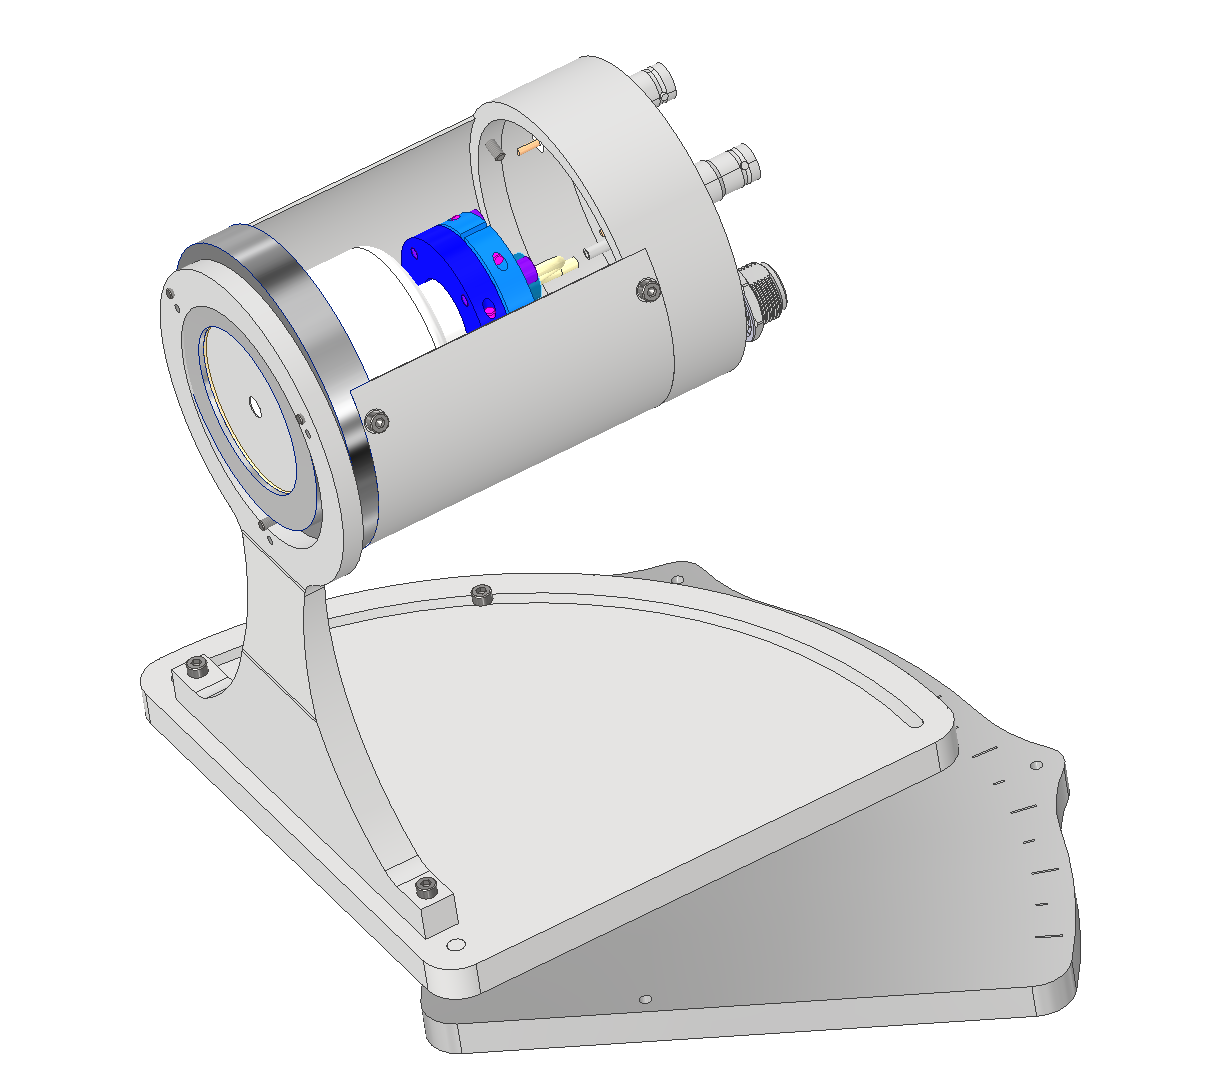
\includegraphics[height=5.9cm,width=\linewidth,keepaspectratio]{img/halterung.png}
    \end{column}
    \begin{column}{\textspalte}
      \begin{itemize}
        \item Unterteil und RIT-Erhöhung auf gemeinsamer Teflonplatte
        \item Achshöhe RFN und RIT gleich, \SI{158}{\milli\meter} über der Platte
        \item Drehscheibe trägt die Frontplatte, Frontplatte trägt den RFN
        \item Frontplatte aus Edelstahl, übrige Teile Aluminium
        \item Langlöcher in der Teflonplatte: RIT \textpm\SI{27}{\milli\meter}, RFN \textpm\SI{8.3}{\milli\meter}
      \end{itemize}
    \end{column}
  \end{columns}
\end{frame}

% ============================================================
\begin{frame}[c]{Drehbarkeit: Stift, Skala, Klemmung}
  \begin{columns}[c]
    \begin{column}{\bildspalte}
      \centering
      \includegraphics[height=5.9cm,width=\linewidth,keepaspectratio,%
                       trim=36 207 523.4 72,clip,page=2]%
        {img/RFN_neu/aufhaengung_zeichnungen.pdf}
    \end{column}
    \begin{column}{\textspalte}
      \begin{itemize}
        \item Drehscheibe dreht auf eingepresstem Zylinderstift \o\,5, Gleitsitz E8 auf m6
        \item Skala im Unterteil von 80\textdegree\ bis 180\textdegree, Teilung 5\textdegree, Zusatzstrich bei 135\textdegree
        \item Drei Zeigerkerben in der Drehscheibe bei 90\textdegree, 135\textdegree, 180\textdegree
        \item Klemmung mit 3 Schrauben M3 durch ein Bogenlangloch, in jeder Stellung
        \item Gleitfläche eben 0,05 und Ra 1,6, damit die Scheibe sauber läuft
      \end{itemize}
    \end{column}
  \end{columns}
\end{frame}

% ============================================================
\begin{frame}[c]{RFN an der Frontplatte}
  \begin{columns}[c]
    \begin{column}{\bildspalte}
      \centering
      \includegraphics[height=5.9cm,width=\linewidth,keepaspectratio,%
                       trim=36 390.7 662.5 57.6,clip,page=4]%
        {img/RFN_neu/aufhaengung_zeichnungen.pdf}
    \end{column}
    \begin{column}{\textspalte}
      \begin{itemize}
        \item Unterring \o\,80 g6 zentriert in \o\,80 H7 der Frontplatte
        \item Eingepresster Stift \o\,2 bei 140\textdegree\ gibt die Drehlage vor
        \item 8 Schrauben M2 auf Lochkreis \o\,84, alle 40\textdegree, Position 140\textdegree\ bleibt für den Stift frei
        \item Verschraubung von vorn, RFN als Ganzes abnehmbar
      \end{itemize}
    \end{column}
  \end{columns}
\end{frame}

% ============================================================
\begin{frame}{Stand und offene Punkte}
  \vfill
  \centering
  \begin{itemize}
    \item Comsol nutzt teilweise alte Geomtrie
    \item Einige neue Simulationen zur Abschätzung der erwartbaren Änderungen
    \item Fertigung der Teile in der Werkstatt
    \item Zusammenbau und Test im Obelix
  \end{itemize}
  \vfill
\end{frame}

% ============================================================
{
\setbeamertemplate{footline}{}
\begin{frame}[plain,c]
  \begin{tikzpicture}[remember picture, overlay]
    \node[anchor=north west, inner sep=0pt] at ([xshift=0.9cm,yshift=-0.6cm]current page.north west)
      {
\includegraphics[height=1.0cm]{img/JLU_Giessen-Logo.pdf}};
    \draw[giessenblau, line width=0.8pt] ([yshift=-1.7cm]current page.north west) -- ([yshift=-1.7cm]current page.north east);
    \draw[giessenblau, line width=0.8pt] ([yshift=1.6cm]current page.south west) -- ([yshift=1.6cm]current page.south east);
  \end{tikzpicture}
  \begin{center}
    {\LARGE\bfseries\color{giessenblau} Vielen Dank}\\[0.8em]
    {\Large\color{grauton} Fragen?}
  \end{center}
\end{frame}
}

\end{document}
